

\section{Strategy Builder}

The Strategy Builder is a key feature of the ezTrading platform, enabling users to create algorithmic trading bots in a low-code setting. The principal attributes of this feature are as follows:
\begin{itemize}
    \item Provides a visual drag-and-drop interface for low-code trading strategy designing.
    \item Allows users to place and connect `State' and `Transition' elements.
    \item `State' elements contain `Task' blocks that describe processes.
    \item `Transition' elements house `Rule' blocks that describe conditions.
    \item Real-time validation and error checking.
\end{itemize}

\subsection{Strategy Builder UI Layout}

The user interface of the Strategy Builder has been carefully designed to offer an intuitive and efficient experience for both novice and expert traders. The layout is organized into several key sections to facilitate easy navigation and task completion.

\subsection{Canvas Area}

The central part of the UI, referred to as the `Canvas Area,' serves as the workspace where users can drag-and-drop `State' and `Transition' elements to construct their trading strategy. This area supports zooming and panning for a more flexible user experience. Additionally, a grid option is available on the canvas, along with features for snapping to the grid and to other objects.

\subsection{Panels and Menus}
\subsubsection{Element Toolbar}

Located on the left-hand side of the screen, the `Element Toolbar' contains a selection of available `State' and `Transition' elements. Users can simply drag an element from this toolbar onto the canvas area to include it in their strategy. The list of available tools in the toolbar is listed below:

\begin{itemize}
  \item \textbf{Viewport}: Select \svgicon{assets/icons/select.svg}, Pad \svgicon{assets/icons/pan.svg}, and Zoom \svgicon{assets/icons/zoom-in.svg} functionalities.
  \item \textbf{Decoration}: Some non-functional objects including Rich Text \svgicon{assets/icons/text.svg}, Image \svgicon{assets/icons/image.svg}, and Shapes \svgicon{assets/icons/shapes.svg} (including basic geometric shapes).
  \item \textbf{Favorites}\svgicon{assets/icons/fav.svg}: A list of selected `Task' and `Rule' block objects.
  \item \textbf{State} \svgicon{assets/icons/state.svg}: A new `State' node.
  \item \textbf{Transition} \svgicon{assets/icons/trans.svg}: A new `Transition' node.
  \item \textbf{Tasks} \svgicon{assets/icons/tasks.svg}: Display the `Tasks' panel. This option can be replaced with an overlay `Add' button \svgicon[0]{assets/icons/add.svg} inside the `State' nodes.
  \item \textbf{Rules} \svgicon{assets/icons/rule.svg}: Display the `Rules' panel. This option can be replaced with an overlay `Add' button \svgicon[0]{assets/icons/add.svg} inside the `Transition' nodes.
\end{itemize}

The `Task' and `Rule' blocks are dynamically defined in form of a JSON file which is obtainable using the \code{/elements} endpoint. See section~\ref{sec:json-elements} for the details of the JSON payload.

\subsubsection{Property Panel}

Located on the right-hand side of the interface, the `Property Panel' houses multiple collapsible sections that facilitate bot customization. 

\begin{itemize}
  \item \textbf{General Settings}: The initial section deals with basic bot settings such as:
  \begin{itemize}
    \item \textbf{Name}: The bot's display name in the list of all bots.
    \item \textbf{Icon}: An optional graphical representation next to the bot's name. If not provided, the system uses the bot's name acronym.
    \item \textbf{Description}: A rich-text editor for describing the bot's functionality, supporting limited formatting options like text color, bold, italics, and so on.
  \end{itemize}

  \item \textbf{Parameters Window}: This section presents a table listing the bot's dynamic parameters, displaying their code-based names, their types, and their UI display names. The window also supports the addition of new parameters and modification of existing ones. Executing either action opens a `Parameter Settings' window, detailed in Section~\ref{sec:parameters}.
  
  \item \textbf{Release Settings}: Here, developers can set the release parameters for the bot, such as:
  \begin{itemize}
    \item \textbf{Date}: The planned release date.
    \item \textbf{Version}: Comprising major, minor, and patch numbers. Must be greater than any previous version.
    \item \textbf{Open-Source}: A checkbox to indicate if the bot is open-source.
    \item \textbf{License}: A drop-down list of licensure options.
    \item \textbf{Price}: The pricing model, either as a one-time fee or a monthly subscription.
    \item \textbf{Trial}: A free trial period in days.
  \end{itemize}

  \item \textbf{Properties Window}: This section adapts according to the selected element on the canvas—be it a `State,' `Transition,' or decorative object. This dynamic panel enables users to edit various properties of the selected element, primarily concerning its appearance. For 'State' elements, additional properties like the name and an `initial state' boolean value can also be modified.
\end{itemize}

Each item in these sections includes an information icon (\svgicon{assets/icons/info.svg}). Hovering over it will pop up a brief explanatory tooltip.


\subsubsection{Top Menu}

The `Top Menu' bar, located at the uppermost part of the UI, offers convenient access to fundamental operations such as creating, saving, loading, and exporting the strategy. This menu bar also accommodates features for undoing and redoing actions. Additionally, an `Execution Box' is integrated into this area, serving as a quick access point for launching backtests, initiating debugging sessions, compiling the code, and publishing the bot.

\subsubsection{Output Console}

Located at the bottom of the UI, the `Output Console' provides real-time logs, warnings, and error messages. This feature helps users troubleshoot their strategies and understand the effects of certain conditions and processes.

\subsubsection{Parameter Settings}
\label{sec:parameters}

The `Parameter Settings' window is invoked from the `Parameters Window' within the `Property Panel' for either adding new parameters or modifying existing ones. This window offers a variety of settings to configure the bot's dynamic parameters.

\begin{table}[h]
\centering
\caption{Data Types for Parameters}
\label{tab:data_types}
\begin{tabular}{|l|l|}
\hline
\textbf{Data Type} & \textbf{Description} \\
\hline
\code{Int} & Whole numbers \\
\hline
\code{Float} & Floating-point numbers \\
\hline
\code{String} & Textual data \\
\hline
\code{Bool} & True or False values \\
\hline
\code{DateTime} & Date and time value \\
\hline
\code{Duration} & Period of time in form of seconds \\
\hline
\code{Symbol} & \begin{tabular}[c]{@{}l@{}}
  Trading symbol of any valid identifier for a\\
  stock, ETF, forex exchange, cryptocurrency, etc.
\end{tabular} \\
\hline
\code{List<Symbol>} & List of symbols \\
\hline
\code{Account} & Brokerage/bank account object \\
\hline
\code{List<Account>} & List of account objects \\
\hline
\code{Enum} & User defined selection list \\
\hline
\end{tabular}
\end{table}

\begin{itemize}
  \item \textbf{Name in Code}: This is the variable name that will be used in the bot's source code to reference the parameter.
  \item \textbf{Display Name}: The name shown in the user interface for the parameter.
  \item \textbf{Data Type}: Defines the type of the parameter. Options are outlined in Table~\ref{tab:data_types}.
  \item \textbf{Default Value}: Specifies an initial value for the parameter. The type of this value must match the selected data type.
  \item \textbf{Minimum and Maximum Values}: Applicable for numerical data types, this setting restricts the range of permissible values.
  \item \textbf{Items}: In case of an \code{Enum} type, this field contains the applicable items.
  \item \textbf{Description}: A text field for providing additional details about the parameter. This will be shown as a tooltip in the user interface.
  \item \textbf{Is Optional}: A checkbox to indicate whether this parameter is optional or mandatory.
\end{itemize}

Once all desired settings have been configured, the user can save the parameter settings, which will then update the parameter list in the `Parameters Window' accordingly.


\subsubsection{Backtesting Panel}
\label{sec:backtest}

The `Backtesting Panel' is a dedicated interface component situated usually on the lower half of the screen. It serves as the central hub for all backtesting-related activities and provides various functionalities that are critical for evaluating trading strategies.

\begin{itemize}
  \item \textbf{Functional Areas}: The panel is divided into several functional areas, each catering to specific needs for backtesting:
  \begin{itemize}
    \item \textbf{Control Buttons}: A series of buttons located at the top of the panel for starting, pausing, and stopping the backtest.
    
    \item \textbf{Time Range}: Controls for selecting the time frame for the backtest, enabling users to test their strategies against historical data within a specified range.
    
    \item \textbf{Settings}: Options for setting initial capital, commissions, and slippage among other simulation parameters.
    
    \item \textbf{Performance Metrics}: A window displaying key performance indicators like Net Profit, Drawdown, and Sharpe Ratio, updated in real-time as the backtest runs.
    
    \item \textbf{Equity Curve}: A graphical representation of the trading account's equity over time.
    
    \item \textbf{Trade Logs}: A tabulated area listing all executed trades, including entry and exit points, as well as profits or losses for each trade.
    
    \item \textbf{Console Output}: An area for displaying any debug messages, errors, or other output generated during the backtest.
  \end{itemize}
  \item \textbf{Interactivity:} Users can interact with the `Backtesting Panel' in several ways:
  \begin{itemize}
    \item Elements in the Performance Metrics window are clickable, providing more detailed statistics upon interaction.
    
    \item The Equity Curve can be zoomed in and out, and specific data points can be hovered over to see precise equity values.
    
    \item Trade Logs offer sorting and filtering options to quickly locate specific trades or to view them according to different criteria.
  \end{itemize}
  \item \textbf{Customization:} One of the key strengths of the `Backtesting Panel' is its customization capabilities. Users can choose which metrics and windows to display, catering the interface to their specific needs and focus.
  \item \textbf{Information Icon:} Each major section within the `Backtesting Panel' has an accompanying information icon \Circled{\textit{i}} that, when hovered over, displays a tooltip providing a brief explanation of the respective functionality.
\end{itemize}

\subsection{Nodes and Elements}

A `Node' is a graphical representation of a computation unit. It can be directly translated into a JSON object to be sent to the server side. Nodes contain `Elements' and can be connected to each other to form a computational sequence. There are two types of nodes in strategy builder environment (Figure~\ref{fig:anatomy}):

\begin{itemize}
  \item \textbf{State Nodes}: These nodes are designed to have multiple inbound and outbound edges, offering users the flexibility to branch out their trading strategy in various directions.
  \item \textbf{Transition Nodes}: In contrast, these nodes are restricted to having only one input and one output. This ensures a streamlined flow of conditions within the strategy.
\end{itemize}

Each node element is draggable and can be deleted. Hovering over the \Circled{?} icon displays an information box, and clicking on it navigates to the corresponding documentation page. Additionally, a `Task' element may feature an \Circled[inner ysep=0.6\baselineskip]{\scriptsize\textbf{=}} icon, allowing developers to assign the task's returned value to a variable.

\begin{figure}
  \caption{The organization of the nodes and elements}
  \label{fig:anatomy}
  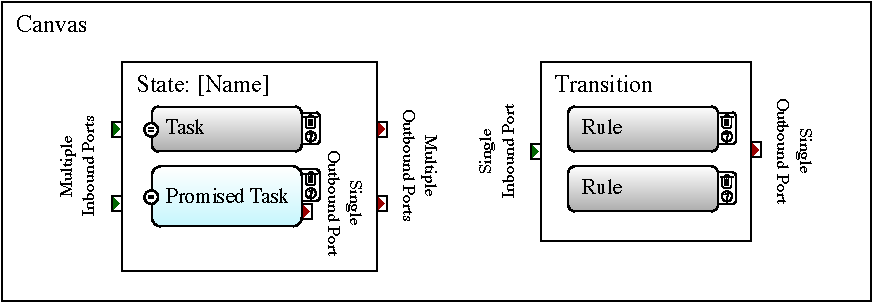
\includegraphics[width=\columnwidth]{assets/Anatomy.pdf}
\end{figure}

\subsubsection{Element Definition}
\label{sec:json-elements}

The frontend fetches the list of available elements by sending a request to the \code{/elements} endpoint, which returns a JSON file as the response. The top level of this JSON file contains two arrays: one for ``tasks'' and another for ``rules,'' as illustrated in Listing~\ref{lst:json-ex}.

\begin{lstlisting}[language=json,firstnumber=1,caption={Sample JSON structure for defining tasks and rules.},label=lst:json-ex]
{
  "tasks": [
    {
      "name": "Task Name",
      "id": 0,
      "icon": "/path/to/svg",
      "keywords": [...],
      "contents": [...],
      "arms": 0,
      "return": "void" | "type" | "promise<type>"
    },
    {
      "name": "Group Name",
      "icon": "/path/to/svg",
      "submenu": [...]
    }
  ],
  "rules": [...]
}
\end{lstlisting}

Each entry in the JSON file must include a \code{"name"}, an \code{"id"}, an \code{"icon"}, and a numeric value denoting the number of \code{"arms"}. Additionally, a set of \code{"keywords"} aids in the search functionality when looking up a `Task' or `Rule'. Entries representing a group of components may include a \code{"submenu"}, as shown in Figure~\ref{fig:grouped-items} where the item ``Loops'' incorporates a submenu.

\begin{figure}[!ht]
\ffigbox[\textwidth]{%
  \begin{subfloatrow}
    \ffigbox[\FBwidth][]
      {\caption{The item `Loops' uses \code{"submenu"} to group multiple components.}\label{sfig:grouped-items}}
      {\includesvg[height=4in]{assets/group.svg}\hspace{1cm}}
  \end{subfloatrow}\hspace*{\columnsep}
  \begin{subfloatrow}
    \vbox{
    \ffigbox[\FBwidth]
      {\caption{A \code{Group} element with unlimited \code{"arms"}.}\label{sfig:group}}
      {\includesvg[height=1.2in]{assets/grouped.svg}}\vss
    \ffigbox[1.5\FBwidth]
      {\caption{A \code{Conditional Branch} element with two \code{"arms"}.}\label{sfig:arms}}
      {\vspace{0.25cm}\includesvg[height=0.6in]{assets/if.svg}}\vss
    \ffigbox[1.5\FBwidth]
      {\caption{A `Task' block returning a value. The user can assign it to a variable like \code{p}.}\label{sfig:ret}}
      {\vspace{0.25cm}\includesvg[height=0.35in]{assets/ret.svg}}%
    }%
  \end{subfloatrow}%
  }{\caption{Results of JSON elements: (a) the usage of \code{"submenu"}, (b) a group of elements, (c) an object with multiple \code{"arms"}, and (d) an object with a \code{"return"} value.}\label{fig:grouped-items}}
\end{figure}

The characteristics and behavior of an object on the canvas are defined by its \code{"contents"}, \code{"arms"}, and \code{"return"} fields. A detailed explanation of the \code{"contents"} field can be found in Section~\ref{sec:contents}. The \code{"arms"} field specifies the allowable number of sub-elements for the object. A value of $-1$ signifies an unlimited number of sub-elements, as seen in Figure~\ref{sfig:group}. A value of $0$ indicates no sub-elements are allowed, while any other numeric value restricts the user to specifying up to that many sub-elements, exemplified in Figure~\ref{sfig:arms}. The \texttt{"return"} field, a string value, signifies the return type of the `Task' object, enabling it to produce an output value that can be assigned to a variable, as demonstrated in Figure~\ref{sfig:ret}. Additionally, the \texttt{"return"} field can be set to a \texttt{"promise"} type, in which case the `Task' should be directly connected to a waiting state. It's important to note that this attribute is not applicable to \texttt{Rule} nodes.


\subsubsection{Contents}
\label{sec:contents}

The \texttt{"contents"} field serves as the core component of an element definition, shaping the functionality of objects placed on the canvas and directly translating them to source code. It consists of an array of textual elements, which are arranged consecutively within a block. Together, these elements create a paragraph that delineates the `Task' or the `Rule'. As objects undergo dynamic changes, the enclosing block may automatically adjust its size to accommodate the updated contents. Should the width of the contents surpass a certain threshold, objects will automatically wrap to a new line. The \texttt{"type"} of each element can belong to one of the following categories:

\begin{itemize}
  \item \texttt{"text"}: Displays static, formatted text.
  \item \texttt{"input"}: Allows the user to input a string value, featuring autocomplete capabilities discussed in Section~\ref{sec:code_assistance}.
  \item \texttt{"select"}: Offers a list of predefined options.
  \item \texttt{"mutable"}: Provides a list of options that can dynamically add new elements to the block.
\end{itemize}

A \texttt{"text"} object remains immutable. It permits limited formatting options such as making certain text segments \textbf{bold}, \textit{italic}, \underline{underlined}, or \textcolor{orange}{colored}. The font family and size are fixed. We are open to suggestions regarding this component. One possible approach is to utilize tags like \texttt{<b>} for bold, \texttt{<i>} for italic, \texttt{<u>} for underlining, and \texttt{<c \#RGB>} for specifying colors.

An \texttt{"input"} object permits in-place value modification by the user. Upon clicking, the object transitions into \textit{edit mode}. In this state, an intellisense helper window appears, as depicted in Figure~\ref{fig:variants}-\Circled{2}.

A \texttt{"select"} object offers a static list of options for user selection. These options are specified as an array of strings under the \texttt{"values"} field.

A \texttt{"mutable"} object hosts multiple \texttt{"variants"}, and each variant consists of two fields: \texttt{"name"} and \texttt{"contents"}. The \texttt{"contents"} field allows for nested objects, offering significant flexibility in configuring the properties of an element.

Listing~\ref{lst:json-pat} 

\begin{lstlisting}[language=json,firstnumber=1,caption={The structure of \code{"contents"} object.},label=lst:json-pat]
"contents": [
  {
    "type": "text",
    "value": "Buy "
  },
  {
    "type": "input",
    "value": "???"
  },
  {
    "type": "mutable",
    "variants": [
      {
        "name": "shares",
        "contents": [
          {
            "type": "text",
            "value": " of "
          },
          {
            "type": "input",
            "value": "APPL"
          }
        ]
      },
      ...
    ]
  },
]
\end{lstlisting}


\begin{figure}[!ht]
  \includesvg[width=\textwidth]{assets/pat.svg}
    \caption{Graphical representation of different variants of the object defined in Listing~\ref{lst:json-pat}. Step \Circled{1} shows a static \code{"text"}, step \Circled{2} is a string \code{"input"}, step \Circled{3} represents a \code{"mutable"} object with four variants, the first one of which adds new contents of an \code{"input"} to the `Task' box, when selected, as depicted in step \Circled{4}.}
    \label{fig:variants}
\end{figure}

\subsubsection{Code Assistance: Autocompletion and Linting}
\label{sec:code_assistance}

The development environment leverages two Web Workers to facilitate both autocompletion and linting functionalities. These features are active within the \texttt{"input"} components where users can input code.

For autocompletion, suggestions include parameters of the bot, variables declared in previous `Task' blocks within the same scope, as well as those declared in outer and top-level scopes. If a `Task' block has a \texttt{"return"} type that is an object, the autocompletion also suggests the object's member variables.

Linting operates statically to identify rule violations listed in Table~\ref{tab:linter_rules}. Upon detecting an issue, the problematic code is underlined with a \error{wavy line}. Hovering the cursor over it will display an error message. Concurrently, the list of errors and warnings in the console panel is updated.

\begin{table}[h]
\centering
\caption{Linting Rules}
\label{tab:linter_rules}
\begin{tabular}{|l|p{0.7\linewidth}|}
\hline
Rule & Description \\
\hline
Undefined Variable & A variable is considered undefined within the current scope. \\
\hline
Isolated State & A state node is isolated, meaning it has no incoming edges. \\
\hline
Dead End & A state node, excluding the initial state, has no outgoing edges. \\
\hline
Dangling Promise & A `Task' with an output of type \code{"promise"} is not connected to any state. For example, a BUY order task returns a Promise that is never used to determine whether the order was executed successfully. \\
\hline
Override Promise & A new `Task' follows a `Task' with an output of type \code{"promise"}. \\
\hline
Additional Rules & Further rules to be determined. \\
\hline
\end{tabular}
\end{table}  


\subsection{Managing Strategies}
\label{sec:strategies-management}

The ezTrading platform prioritizes user-friendliness and efficiency in the management of trading bots, aiming to provide an effortless experience for traders at all skill levels. The bots and their associated strategies are securely stored in a backend database, accessible, modifiable, and retrievable through well-defined APIs.

The platform employs three specialized database tables to manage various phases of a trading bot's lifecycle—ranging from its development and publication to user subscriptions. Each table has a unique role in this lifecycle, ensuring robust and secure management procedures.

\subsubsection{Strategy Source Repository}
This table functions as the central store for each bot's developmental assets, including its strategy diagram, source code, and specific version settings. Within the strategy builder UI, developers can browse their projects by clicking the `Projects' button (\svgicon[.3]{assets/icons/projects.svg}). This action opens a new tab, fetching the chosen diagram from the table. Autosave features ensure that any updates to the diagram or source code are consistently saved.

\subsubsection{Published Bot Archives}
Upon rigorous testing and subsequent release into the marketplace, an immutable copy of a bot is stored in this table. While bots in this state cannot be altered, developers can create new versions via the `Clone' button (\svgicon[.3]{assets/icons/clone.svg}) in the source repository table. Additionally, this table houses various statistics and achievements associated with each bot. As stated earlier, an instance of each bot continuously operates in the background with default settings, earning or losing badges over time. This data is stored for quick and precise search functionality.

\subsubsection{User Subscription Records}
This table logs individual user subscriptions to various published bots, alongside the user's personalized settings. Users can modify this table, either by revoking a subscription or by adjusting the settings of a subscribed bot.

\subsection{Version Control in ezTrading}
\label{sec:version-control}

Version Control is an integral aspect of managing trading bot strategies, aimed at facilitating iterative development and collaboration among developers. This feature allows users to manage different versions of a bot, roll back to previous versions, and even branch off to create new variations of an existing bot.

\subsubsection{Versioning Mechanism}
\label{subsec:versioning}

Every time a significant change is made to a bot's strategy diagram or source code, a new version is automatically created. These versions are timestamped and can be programmatically accessed via the platform's API. The history of all versions is displayed in the strategy builder UI, enabling users to easily navigate between different versions and understand the evolution of their bot's strategy.

\subsubsection{Rollback and Recovery}
\label{subsec:rollback}

In case of accidental changes or errors, the Version Control system allows for immediate rollback to a previous state. This feature enhances the robustness and fault-tolerance of the development process, ensuring that errors can be easily rectified.

\subsubsection{Branching and Collaboration}
\label{subsec:branching}

Version Control in ezTrading supports branching, allowing developers to create parallel versions of a bot for experimental features or collaborative work. Each branch can be independently developed and tested before being merged back into the main version. This feature is particularly useful for teams of developers working on complex strategies.

\subsubsection{Audit and Compliance}
\label{subsec:audit}

All changes to a bot, including who made the change and when, are meticulously logged for auditing purposes. This is essential for maintaining a high level of security and compliance, especially for bots that manage significant financial assets.

\subsubsection{Version Control in ezTrading}
\label{sec:version-control-ez}

In ezTrading, version control is entirely optional. We do not provide our own version control system but instead facilitate the integration of third-party version control platforms. Developers who opt to use this feature must connect their own GitHub account, or other version control accounts, to their ezTrading account. If this option is not utilized, we only retain the released versions of a bot upon its publication and maintain a single development copy.

\subsubsection{Mechanism for Third-Party Version Control Integration}
\label{subsubsec:third-party-version-control}

EzTrading offers the capability to integrate with a variety of third-party version control systems such as GitHub, GitLab, and Bitbucket. Here's how the integration works:

\begin{enumerate}
    \item \textbf{OAuth2 Authorization:} Authenticate your ezTrading application with the chosen version control platform using OAuth2. This allows ezTrading to interact with the version control system on behalf of the developer.
    \item \textbf{Repository Management:} Post-authorization, developers can either link to an existing repository or create a new one specifically for their bot strategies.
    \item \textbf{File Operations:} Any significant changes made within the ezTrading platform can be committed and pushed to the repository. This keeps track of different versions and iterations of the bot.
    \item \textbf{Version Navigation:} Developers can fetch and revert to older versions or different branches of their bot strategies as stored in the repository.
    \item \textbf{Collaboration:} Leverage fork and pull request features for team-based development.
    \item \textbf{Event Hooks:} Utilize webhooks to notify of events like new commits or merged pull requests.
    \item \textbf{Audit Trail:} Benefit from detailed logs and history for auditing and tracking purposes.
\end{enumerate}

By integrating a third-party version control system, developers can leverage the benefits of data integrity, security, and collaboration while also enjoying the robust trading capabilities that ezTrading offers.


\subsection{Live Collaboration}
\label{sec:live-collaboration}

Live collaboration in the Strategy Builder UI is one of the standout features that sets ezTrading apart, enabling multiple users to work on a single trading bot strategy simultaneously. This feature mimics the functionalities of well-known collaborative editors, providing real-time synchronization and updates.

\subsubsection{How It Works}
\label{subsubsec:how-it-works}

Upon opening a strategy, a user can invite collaborators by sharing a unique link generated by the system. Once the collaborators join:

\begin{enumerate}
    \item \textbf{Cursor Indicators:} Each user's cursor appears with a unique color, helping to identify individual contributors.
    \item \textbf{Real-time Synchronization:} All changes to the strategy are synchronized in real-time among all active users.
    \item \textbf{Version Merging:} Any conflicts arising from simultaneous edits are smartly resolved to merge versions seamlessly.
    \item \textbf{Chat Support:} A built-in chat system allows for instant communication among team members.
\end{enumerate}

\subsubsection{Permission Levels}
\label{subsubsec:permission-levels}

Collaborators can be assigned varying levels of permissions:

\begin{itemize}
    \item \textbf{Read-only:} Users can view the strategy but not make any changes.
    \item \textbf{Read-Write:} Users can edit the strategy and participate fully in the collaborative process.
    \item \textbf{Admin:} In addition to editing, Admin users can invite or remove collaborators and change permission levels.
\end{itemize}

\subsubsection{Activity Log}
\label{subsubsec:activity-log}

An activity log tracks all changes, additions, and deletions, storing them in a history panel for easy tracking and accountability. Users can revert to prior versions from this panel, ensuring that mistakes can be easily corrected.

\subsubsection{Conflict Resolution}
\label{subsubsec:conflict-resolution}

In case of conflicting changes, a notification prompts the users involved to review the sections in question. A manual override option is available for admin-level collaborators to resolve these conflicts.

By offering live collaboration features, ezTrading ensures a dynamic and interactive strategy development process, facilitating both individual creativity and team-based innovation.
